\documentclass{beamer}

\usetheme{Antibes}
\usepackage{german} 
%\usepackage{beamerthemesplit}
\usepackage{graphicx}
\usepackage{multirow}
\usepackage{multicol}
\usepackage{verbatim}

\title{Diplomarbeit: Objektorientierte Entwicklung eines GUI-basierten Tools f\"{u}r die ereignisbasierte Simulation verteilter Systeme}
\author{Von Paul C. B\"{u}tow\\
~	
\\
1. Pr\"{u}fer: Prof. Dr.-Ing. M. O\ss{}mann\\
2. Pr\"{u}fer: Prof. Dr. rer. nat. H. Fa\ss{}bender}
\date{Fachhochschule Aachen - 18. August 2008}

\begin{document}

\frame{\titlepage}

\newcommand{\elem}[1]{
	\begin{minipage}{.1\linewidth} 
	\centering 
	\includegraphics[scale=.7]{#1}
	\end{minipage} 
}

\section{Einleitung}
\frame{\tableofcontents}

\subsection{Was ist ein verteiltes System?}

\frame{
\frametitle{Was ist ein verteiltes System?}
\begin{itemize}
	\item<1-> Zitat Tanenbaum, van Steen; Verteilte Systeme: ``\textit{Ein verteiltes System ist eine Menge voneinander unabh\"{a}ngiger Computer, die dem Anwender wie ein einzelnes, koh\"{a}rentes System erscheinen}''
	\item<1-> Anwender muss sich nur mit dem vor ihm befindlichen Computer auseinandersetzen
	\item<1-> Verteiltes System stellt die Kommunikation mit anderen Computern sicher 
	\item<1-> Gemeinsame Nutzung von Ressourcen
\end{itemize}
}

\subsection{Motivation}

\frame{
\frametitle{Motivation}
\begin{itemize}
	\item<1-> Betrachtung von verteilten Systemen aus einer anderen Sicht (Lehrzwecke)
	\item<1-> Transparente Darstellung von verteilten Systemen
	\item<1-> Entwicklung eines Simulators (VS-Simulator oder auch VS-Sim.)
		\begin{itemize}
			\item<1-> Flexibilit\"{a}t
			\item<1-> Einfachheit in der Bedienung
			\item<1-> Erweiterungsm\"{o}glichkeiten
		\end{itemize}
\end{itemize}
}

\section{Grundlagen}

\subsection{Client/Server}

\frame{
\frametitle{Grundlagen - Client/Server}
\begin{itemize}
	\item<1-> Client/Server Kommunikation
	\item<1-> Mindestens einen Client und einen Server
	\item<1-> Verschicken von Nachrichten
		\begin{itemize}
			\item<1-> Client kann nur Servernachrichten verarbeiten
			\item<1-> Server kann nur Clientnachrichten verarbeiten
		\end{itemize}
\end{itemize}
\begin{center}
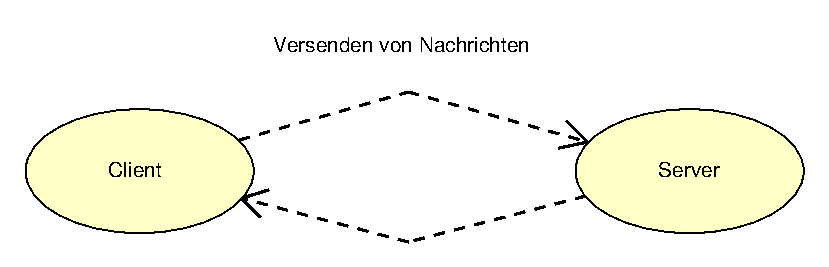
\includegraphics[scale=.5]{client-server}
\end{center}
}
\subsection{Prozesse}

\frame{
\frametitle{Grundlagen - Prozesse}
\begin{itemize}
	\item<1-> Simulation von (beliebig vielen) verteilten Prozessen
	\item<1-> Jeder Prozess kann Rollen einnehmen
		\begin{itemize}
			\item<1-> Prozess ist Server
			\item<1-> Prozess ist Client
			\item<1-> oder Prozess ist gleichzeitig Client und Server
		\end{itemize}
\end{itemize}
} 

\subsection{Protokolle}

\frame{
\frametitle{Protokolle}
\begin{itemize}
	\item<1-> Ein Protokoll definiert das Verhalten von Clients und Severn
		\begin{itemize}
			\item<1-> Was in den Nachrichten verschickt wird
			\item<1-> Wie auf den Erhalt einer Nachricht reagiert wird
			\item<1-> Was bei Wecker-Ereignissen passiert
		\end{itemize}
\end{itemize}
} 

\frame{
\frametitle{Protokolle}
\begin{itemize}
	\item<1-> Jede Nachricht geh\"{o}rt einem Protokoll an
		\begin{itemize}
			\item<1-> Nachricht nur verarbeitbar, wenn Empf\"{a}nger das Protokoll der Nachricht versteht
			\item<1-> Alle anderen eintreffenden Nachrichten werden nicht verarbeitet
		\end{itemize}
\end{itemize}
} 

\subsection{Uhren}

\frame{
\frametitle{Uhren und Zeit}
\begin{itemize}
	\item<1-> Simulation hat eine globale Uhr
	\item<1-> Jeder Prozess hat:
		\begin{itemize}
			\item<1-> Eigene Prozessuhr / Uhrabweichung
			\item<1-> Lamport-Zeitstempel
			\item<1-> Vektor-Zeitstempel
		\end{itemize}
\end{itemize}
} 

\subsection{Ereignisse}

\frame{
\frametitle{Ereignisse}
\begin{itemize}
	\item<1-> Simulation: Hintereinanderausf\"{u}hrung von Ereignissen
	\item<1-> Ereignis bei lokaler Prozesszeit oder globaler Zeit
		\begin{itemize}
			\item<1-> Prozessabsturz/Prozesswiederbelebung
			\item<1-> Aktivierung oder Deaktivierung eines Protokolls client- oder serverseitig 
			\item<1-> Starten von Client- bzw. Serveranfragen
		\end{itemize}
	\item<1-> Weitere (interne) Ereignisse
		\begin{itemize}
			\item<1-> Zuf\"{a}llige Ereignisse
			\item<1-> Wecker-Ereignisse
			\item<1-> Nachrichtenempfangs-Ereignisse
		\end{itemize}
\end{itemize}
} 

\section{Der Simulator}

\subsection{Konfigurationsm\"{o}glichkeiten}

\frame{
\frametitle{Verschiedene Einstellungsm\"{o}glichkeiten}
\begin{itemize}
	\item<1-> Vom Anwender einstellbar und abspeicherbar
	\begin{itemize}
		\item<1-> Globale Simulationseinstellungen
		\item<1-> Separate Einstellungen f\"{u}r jeden Prozess
		\item<1-> Separate Einstellungen f\"{u}r jedes Protokoll f\"{u}r jeden Prozess
	\end{itemize}
	\item<1-> Vom Entwickler einstellbar
	\begin{itemize}
		\item<1-> \texttt{prefs/VSDefaultPrefs.java}
		\item<1-> Alle Standardeinstellungen
		\item<1-> Spracheinstellungen
	\end{itemize}
\end{itemize}
} 

\subsection{Alle bereits eingebauten Protokolle}

\frame{
\frametitle{Derzeit verf\"{u}gbare Protokolle}
\begin{itemize}
	\item<1-> Das Beispiel (Dummy) Protokoll
	\item<1-> Das Ping-Pong Protokoll
	\item<1-> Das Broadcast Protokoll
	\item<1-> Das Protokoll zur internen Synchronisierung in einem synchronen System
	\item<1-> Das Protokoll zur Christians Methode zur externen Synchronisierung
	\item<1-> Der Berkeley Algorithmus zur internen Synchronisierung
	\item<1-> Das Ein-Phasen Commit Protokoll 
	\item<1-> Das Zwei-Phasen Commit Protokoll 
	\item<1-> Der ungen\"{u}gende (Basic) Multicast
	\item<1-> Der zuverl\"{a}ssige (Reliable) Multicast
\end{itemize}
} 

\subsection{Beispiele / Vorf\"{u}hrungen}

\frame{
\frametitle{Beispiele}
\begin{itemize}
	\item<1-> Das Beispiel (Dummy) Protokoll
	\item<1-> Das Ping-Pong Protokoll
	\item<1-> Ping-Pong Sturm
	\item<1-> Das Protokoll zur Christians Methode zur externen Synchronisierung \textit{(wenn genug Zeit)}
	\item<1-> Der zuverl\"{a}ssige (Reliable) Multicast \textit{(wenn genug Zeit)}
\end{itemize}
} 

\subsection{Implementierung von Protokollen (Protokoll-API)}

\frame{
\frametitle{Ereignisse und Protokolle / Klassenvererbungen}
	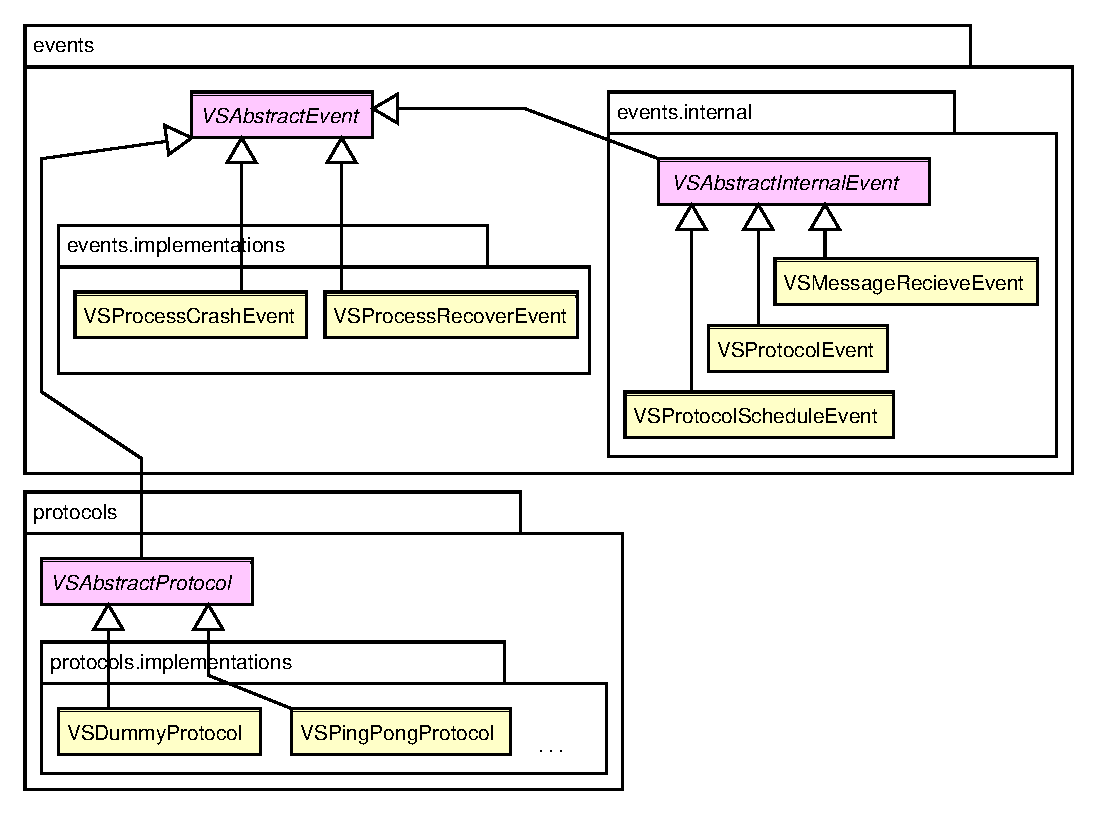
\includegraphics[scale=.5]{vererbungen}
} 

\frame{
\frametitle{Methoden einer Protokollklasse}
\begin{itemize}
	\item<1-> \texttt{public VSDummyProtocol()} (Konstruktor)
	\item<1-> \texttt{public void onClientInit()}
	\item<1-> \texttt{public void onClientReset()}
	\item<1-> \texttt{public void onClientStart()}
	\item<1-> \texttt{public void onClientRecv(VSMessage message)}
	\item<1-> \texttt{public void onClientSchedule()}
	\item<1-> \texttt{public void onServerInit()}
	\item<1-> \texttt{public void onServerReset()}
	\item<1-> \texttt{public void onServerStart()}
	\item<1-> \texttt{public void onServerRecv(VSMessage message)}
	\item<1-> \texttt{public void onServerSchedule()}
\end{itemize}
} 

\frame{
\frametitle{Geerbte Methoden und Attribute}
\begin{itemize}
	\item<1-> Geerbte Attribute
	\begin{itemize}
		\item<1-> \texttt{protected VSAbstractProcess process}
		\item<1-> \texttt{protected VSPrefs prefs}
	\end{itemize}
	\item<1-> Geerbte Methoden
	\begin{itemize}
		\item<1-> \texttt{public void log()}
		\item<1-> \texttt{public String toString()}
		\item<1-> \texttt{public void sendMessage(VSMessage message)}
		\item<1-> \texttt{public void scheduleAt(long time)}
		\item<1-> \texttt{public void removeSchedules()}
		\item<1-> ... und viele mehr
	\end{itemize}
\end{itemize}
} 

\section{Ende}

\subsection{Ausblick}

\frame{
\frametitle{Denkbare Erweiterungen}
\begin{itemize}
	\item<1-> Wahrscheinlich Ver\"{o}ffentlichung als Open Source
	\item<1-> Neue Ereignisse und Protokolle
	\item<1-> Erweiterungen als Plugins 
	\item<1-> Beliebig lange Simulationen 
	\item<1-> Scroll- und Zoomfunktionen
	\item<1-> Ereignisse bei Lamport- und Vektor-Zeitstempel
	\item<1-> ... und vieles mehr
\end{itemize}
} 

\subsection{Zahlen und Fakten}

\frame{
\frametitle{VS-Sim.: Zahlen und Fakten}
\begin{itemize}
	\item<1-> Quelltext-Dateien: 61
	\item<1-> Java-Pakete: 12 
	\item<1-> LOC: 15710 
	\item<1-> Generierte Javadocs: 2.2MB 
	\item<1-> VS-Sim-1.0.jar: 142KB
	\item<1-> Bereits eingebaute Protokolle: 10
	\item<1-> Einstellungsm\"{o}glichkeiten: 163 (ohne Protokolle)
\end{itemize}
} 

\frame{
\frametitle{Danke f\"{u}r die Aufmerksamkeit}
\begin{itemize}
	\item<1-> Quelltext-Dateien: 61
	\item<1-> Java-Pakete: 12 
	\item<1-> LOC: 15710 
	\item<1-> Generierte Javadocs: 2.2MB 
	\item<1-> VS-Sim-1.0.jar: 142KB
	\item<1-> Bereits eingebaute Protokolle: 10
	\item<1-> Einstellungsm\"{o}glichkeiten: 163 (ohne Protokolle)
\end{itemize}
} 

\end{document}
    
